\documentclass{article}
\usepackage{graphicx} % Required for inserting images
\usepackage[utf8]{inputenc}
\usepackage[french]{babel} %Pour les accents.
\usepackage{amssymb} %Pour les corps.
\usepackage{stmaryrd} %Pour les doubles crochets (intervalles entiers).
\usepackage{enumitem} %Pour énumérer avec autre chose que 1,2,3.
\usepackage{amsmath} %Pour les coefs binomiaux.
\usepackage{float}
\usepackage{array}
\usepackage{listings}
\usepackage[left=2cm,right=2cm,top=2cm,bottom=2cm]{geometry} %Pour régler la taille de la marge.
\usepackage[T1]{fontenc}
\setlength\parindent{0pt}
\usepackage{booktabs}
\usepackage{float}
\usepackage{hyperref}
\hypersetup{
    colorlinks=true,
    linkcolor=blue,
    filecolor=magenta,      
    urlcolor=cyan,
}
\usepackage{easytable}
\usepackage{adjustbox}
\usepackage{tikz,lipsum,lmodern}
\usepackage[most]{tcolorbox}

\newcommand{\bZ}{\mathbb{Z}}

\newcommand{\bun}{\mathbf{1}}
\newcommand{\bN}{\mathbb{N}}
\newcommand{\bR}{\mathbb{R}}
\newcommand{\bP}{\mathbb{P}}
\newcommand{\bE}{\mathbb{E}}
\newcommand{\bV}{\mathbb{V}}
\newcommand{\bF}{\mathbb{F}}
\newcommand{\bQ}{\mathbb{Q}}
\newcommand{\intbrac}[2]{\llbracket #1,#2\rrbracket}
\newcommand{\Prin}{\operatorname{Prin}}
\newcommand{\Pic}{\operatorname{Pic}}
\newcommand{\Diag}{\operatorname{Diag}}
\usepackage[backend=biber]{biblatex}
\addbibresource{ref.bib}

\usepackage{fancyhdr}
\usepackage{setspace}
\usepackage{lastpage}
\usepackage[most]{tcolorbox}
\newcommand{\HRule}{\rule{\linewidth}{0.5mm}}

\pagestyle{fancy}
\renewcommand\headrulewidth{1pt}
\renewcommand\footrulewidth{1pt}
\geometry{headsep=1.1cm}

\fancyhead[L]{
\includegraphics[width=0.1\columnwidth]{./logo}~}
\fancyfoot[L]{\textsc{Algèbre \& Cryptologie
}}
\fancyhead[R]{\textsc{Challenge 4}}
\fancyfoot[C]{\thepage/\pageref{LastPage}}
\fancyfoot[R]{\textsc{\today}}

\title{Algèbre \& Cryptologie : Challenge 2}
\author{Raphaël PAIN DIT HERMIER\\
Alexis LOMBARD-GAILLARD\\
Edward LUCYSZYN}
\date{Avril 2024}

\begin{document}

\begin{titlepage}
\begin{center}

% Upper part of the page. The '~' is needed because only works if a paragraph has started.

\LARGE \textsc{2EL1740: Algèbre \& Cryptologie}

\vspace{0.2cm}

\Large \textsc{CentraleSupélec - 2A}

\vspace{0.3cm}

% Title
\HRule \\[0.4cm]

{\huge \bfseries Challenge 4\\
[0.2cm]}

\HRule \\[0.4cm]

\vspace{2cm}

\textsc{\today}

\vspace{2cm}


\includegraphics[width=0.4\columnwidth]{./logo}~\\[3cm]

% Author and supervisor
\begin{minipage}{0.4\textwidth}
\begin{spacing}{1.125}
\begin{center}
    Raphaël \testsc{PAIN DIT HERMIER}\\
    Alexis \testsc{LOMBARD-GAILLARD}\\
    Edward \testsc{LUCYSZYN}
\end{center}
\end{spacing}
\end{minipage}

\vfill

\end{center}
\end{titlepage}

\tableofcontents

\newpage
\section{Question 1}

On considère l'équation
\[(E): \quad y^3 = x^2-7,\]
dont on cherche les solutions d'abord dans $\bZ$, dans $\bF_p$ avec $p = 2^{123}+165$, puis dans $\bQ$.

\subsection{Résolution dans $\bZ$ et $\bQ$}

On considère d'abord $(E)$ comme une équation à résoudre sur $\bZ$.\\

Utilisons SageMath pour se représenter la courbe $(E)$. On réécrit l'équation sous la forme $(E): x^2 = y^3+7$ On modélise alors la courbe $(F): y^2 = x^3+7$, qui n'est rien d'autre que la courbe $(E)$ réfléchie selon la droite $y=x$. $(F)$ est bien une courbe elliptique lisse car $\Delta E = 27\times 7^2 = 1323 \neq 0$. Dans SageMath, on écrit les lignes de code suivantes pour se donner une idée des solutions :

\begin{lstlisting}[language = Python]

F = EllipticCurve(QQ, [0, 0, 0, 0, 7])
F.gens()
F.integral_points()

\end{lstlisting}

\begin{figure}[h]
\centering
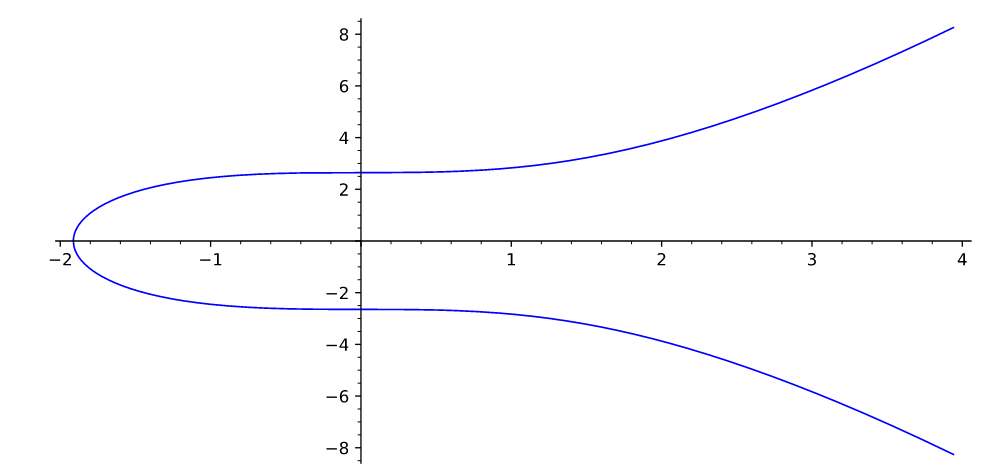
\includegraphics[width=0.7\textwidth]{Capture d'écran 2024-05-22 151712.png}
\caption{Courbe elliptique $y^2 = x^3+7$ tracée sur $\bR$.}
\label{fig:exemple}
\end{figure}

Les commandes "F.gens()" et "F.integral\_points()" nous renvoient des listes vides, suggérant qu'il n'existe ni de solutions dans $\bZ$, ni dans $\bQ$. Pour s'en assurer, prouvons cette conjecture mathématiquement, premièrement dans $\bZ$.\\

Commençons par énoncer et prouver le résultat suivant, qui nous permettra d'affirmer que $\bZ[\sqrt{7}]$ est un anneau de Dedekind :

\begin{tcolorbox}[colback=red!5!white,colframe=red!75!black,title=Théorème : Anneau d'entiers d'un corps de nombres quadratique]
    Soit $d\in \bZ\backslash \{0,1\}$ sans facteur carré. Alors l'anneau d'entiers de $\bQ(\sqrt{d})$ est
    \[\bZ[\alpha] = \{a+b\alpha | a,b\in \bZ\}\]
    où
    \[\alpha = \begin{cases}
        \sqrt{d}& \text{ si } d\equiv 2\text{ ou }3[4],\\
        \frac{1+\sqrt{d}}{2} & \text{ si } d\equiv 1[4].
    \end{cases}\]
\end{tcolorbox}
    \textbf{Preuve :}  Soit \( x = a + b\sqrt{d} \in K \) où \( (a, b) \in \mathbb{Q}^2 \). Déterminons une condition nécessaire pour que \( x \in \mathcal{O}_K \). Posons \( \overline{x} = a - b\sqrt{d} \). Comme \( \overline{x} \) est un conjugué de \( x \), il s’agit d’un entier algébrique (car $x$ et $\overline{x}$ ont le même polynôme minimal). Par ailleurs le polynôme
\[ P(X) = (X - x)(X - \overline{x}) = X^2 - (x + \overline{x})X + x\overline{x} \]
est à coefficients dans \(\mathbb{Q}\). De plus, ses coefficients \( x + \overline{x} \) et \( x\overline{x} \) sont également des entiers algébriques. Comme les seuls entiers algébriques de \(\mathbb{Q}\) sont les éléments de \(\mathbb{Z}\), on en déduit donc que
\[ x + \overline{x} \in \mathbb{Z}, \quad x\overline{x} \in \mathbb{Z}. \]
On a donc \( 2a \in \mathbb{Z} \) et \( a^2 - db^2 \in \mathbb{Z} \). Posons \( a_1 = 2a \in \mathbb{Z} \) de sorte que \( a_1^2 - 4db^2 \in 4\mathbb{Z} \). On en déduit que \( 4db^2 \in \mathbb{Z} \). Soit \( p \) un nombre premier. On déduit de cette relation la relation
\[ v_p(4) + v_p(d) + 2v_p(b) \geq 0. \]
Comme \( d \) est sans diviseur carré, on a \( v_p(d) \in \{0, 1\} \) de sorte que, si \( p \ne 2 \), on a \( v_p(b) \geq 0 \) et, si \( p = 2 \), \( v_2(b) \geq -1 \). On en déduit la relation \( 2b \in \mathbb{Z} \). Posons donc \( b_1 = 2b \). La relation \( a_1^2 - db_1^2 \in 4\mathbb{Z} \) et le fait que \( d \) est sans diviseur carré implique que \( 2 \) divise \( a_1 \) si et seulement si \( 2 \) divise \( b_1 \). On en déduit que si \( 2 \) ne divise pas \( a_1 \), alors \( 2 \) ne divise pas \( b_1 \) et on obtient donc
\[ d = a_1^2b_1^{-2} \text{ dans } \mathbb{Z}/4\mathbb{Z}. \]
En particulier, \( d \) est un carré modulo 4. Comme \( d \) est sans diviseur carré, on a \( d \ne 0 \) et donc \( d \equiv 1 [4] \). Ainsi, si \( d \) est congru à 2 ou 3, modulo 4, les entiers \( a_1 \) et \( b_1 \) sont tous deux pairs et donc \( (a, b) \in \mathbb{Z}^2 \). En particulier \( x \in \mathbb{Z}[\sqrt{d}] \). Si \( d \equiv 1 \pmod{4} \), alors \( a_1 \) et \( b_1 \) ne sont pas nécessairement pairs mais ont nécessairement la même parité. On en déduit que \( (a, b) \in \left(\frac{1}{2}\mathbb{Z}\right)^2 \) avec \( a - b \in \mathbb{Z} \). En particulier \( x \in \mathbb{Z}\left[\frac{1 + \sqrt{d}}{2}\right] \).

Réciproquement, posons \( \alpha = \frac{1 + \sqrt{d}}{2} \) si \( d \equiv 1 [4] \), et \( \alpha = \sqrt{d} \) dans le cas contraire. Il nous reste à vérifier que les éléments de \( \mathbb{Z}[\alpha] \) sont bien des entiers algébriques. D’après le corollaire au théorème 5.1, il est suffisant de vérifier que \( \alpha \) est un entier algébrique. Le nombre \( \sqrt{d} \) est toujours un entier algébrique puisqu’il est annulé par le polynôme unitaire \( X^2 - d \in \mathbb{Z}[X] \). Le polynôme minimal du nombre \( \frac{1 + \sqrt{d}}{2} \) est le polynôme
\[ \left( X - \frac{1 + \sqrt{d}}{2} \right) \left( X - \frac{1 - \sqrt{d}}{2} \right) = X^2 - X + \frac{1 - d}{4} \]
    Qui est bien à coefficients entiers lorsque $d\equiv 1[4]$. $\square$\\

Ici on prend $d = 7$, donc $d\equiv 3[4]$ et $\bZ[\sqrt{7}]$ est un anneau d'entiers, donc de Dedekind. Cela implique la factorisation unique en idéaux premiers. On admettra que le groupe d'idéaux de $\bZ[\sqrt{7}]$ est de taille $2$.\\


Apportons alors la réponse à notre question de départ. Supposons $(x,y)\in \bZ^2$ solution de $(E)$.\\
Si par l'absurde $x = 7k$ avec $k\in \bZ$, alors $y^3 = 7(7k-1)$, donc $7|y^3$. Comme $7$ est premier, le lemme de Gauss implique que $7|y$. Donc $7^3|y^3$, soit que $7^2|(7k-1)$. Or $7k-1\equiv -1[7]$, ce qui est absurde.\\
Donc $x$ n'est pas un multiple de $7$. Par suite, on remarque l'égalité d'idéaux dans $\bZ[\sqrt{7}]$:
\[(y)^3 = (x-\sqrt{7})(x+\sqrt{7}).\]

Comme $x$ n'est pas un multiple de $7$ et que $7$ est premier, on peut se munir d'un couple de Bézout $(u,v)$, tel que $ux + 7v = 1$.
Pour trouver $a,b,c,d$ entiers tels que $(a+b\sqrt{7})(x+\sqrt{7}) + (c+d\sqrt{7})(x-\sqrt{7}) = 1$, il suffira de les prendre tels que $a+c = u$, $b-d = v$ et $(a-c) + (b+d)x = 0$.\\
Ceci nous conduit au fait que les idéaux $(x-\sqrt{7})$ et $(x+\sqrt{7})$ sont premiers entre eux.\\

Par factorisation unique, $(x-\sqrt{7})$ est forcément un cube d'idéal, i.e il existe un idéal $I$ tel que $I^3 = (x-\sqrt{7})$. Si par l'absurde $I$ n'est pas principal, alors $I^3$ ne l'est pas non plus car le groupe d'idéaux de $\bZ[\sqrt{7}]$ est de taille $2$. C'est absurde car $I^3 = (x-\sqrt{7})$.\\
Donc $I$ est principal et on écrit $I = (a+b\sqrt{7})$ pour un certain couple $(a,b)\in \bZ^2$. Or $I^3 = \left((a+b\sqrt{7})^3\right) = (a^3+7ab^3 + b(a^2 + 7b^2)\sqrt{7})$. On en déduit que $b(a^2+7b^2) = \pm 1$. Par calcul dans $\bZ$, $b = \pm 1$, ainsi aucune valeur de $a$ n'est satisfaisante.
On en conclut qu'il n'existe aucune solution dans $\bZ$.\\

Supposons maintenant par l'absurde qu'il existe un couple $(a,b)$ solution de $(E)$ sur $\bQ$. Quitte à multiplier les dénominateurs, on peut écrire $\displaystyle a = \frac{x}{q^3}$ et $\displaystyle b = \frac{y}{q^2}$ pour des certains $x,y\in \bZ$ et $q\in \bN^*$. Alors $(x,y)$ est solution entière de l'équation \[(E_q) : y^3 = x^2 - 7q^6.\]

Supposons d'abord $x$ est multiple de $7$. Alors par un raisonnement similaire à celui fait dans $\bZ$, si $x = 7x_1$ et $y = 7y_1$, alors $7^2|(7x_1^2 + q^6)$, donc forcément $7|q$, soit $q = 7q_1$. Puis $7|(x_1^2 + 7^5q_1^6)$. donc $7|x_1$, si bien que $x_1 = 7x_2$. Donc $y_1^3 = 7x_2^2 - 7^4q_1^6$, et $7|y_1$, si bien que $y_1 = 7y_2$. Donc $7^2|(x_2^2-7^3q_1^6)$, si bien que $x_2 = 7x_3$. On obtient alors que $y_2^2 = x_3^3 - 7q_1^6$.\\ \\
Ainsi on vient de voir, quitte à diviser par des puissances de 7, qu'on peut toujours créer une solution $(x,y)\in \bZ^2$ à une équation elliptique du type $(E_q)$ où $x$ n'est pas un multiple de $7$.\\
On peut alors appliquer le même raisonnement par factorisation d'idéaux dans $\bZ[\sqrt{7}]$ (on aura alors $(y)^3 = (x-q^3\sqrt{7})(x+q^3\sqrt{7})$) pour trouver qu'une telle solution $(x,y)$ est impossible.\\ \\
On a finalement prouvé par l'absurde qu'il n'existe aucune solution dans $\bQ$.


\subsection{Résolution dans $\bF_p$}

On cherche maintenant les solutions de $(E)$ dans $\bF_p$, où $p = 2^{123}+165$.\\

On vérifiera pour s'assurer que $2^{123}+165$ est un nombre probablement premier, grâce à des outils comme la fonction python "isprime" ou notre test de Miller-Rabin (challenge 1), et ce dernier renvoie que $p$ est bel et bien probablement premier.\\

On ressort la courbe symétrique $F : v^2 = u^3 + 7$, ce qui est la forme de Weierstrass courte d'une équation elliptique lisse sur $\bQ$. Puis comme $\Delta E = 1323$, il est clair que $p\nmid \Delta F$, si bien que $F$ a bonne réduction sur $\bF_p$.

On considère le polynôme $P:(x,y,z)\in \mathbb{P}^2\bF_p \longmapsto u^3 - v^2w + 7w^3$, qui est bien un polynôme homogène. De plus, $|\mathbb{P}^2\bF_p| = p^2+p+1 < 2^{128}$, donc nous pouvons facilement calculer le groupe engendré par la courbe elliptique avec SageMath.

\begin{lstlisting}[language = Python]

G = Zmod(2^123 + 165)
F2 = EllipticCurve(G, [0, 0, 0, 0, 7])
F2.abelian_group()
F2.gens()

\end{lstlisting}

Ce code nous renvoie que la courbe $F$ considérée sur $\bP^2\bF_p$ représente un groupe abélien de cardinal\\$10633823966279326983230456482242756774 = p+1$, et qu'en plus ce groupe est cyclique. Donc le groupe est isomorphe à $\bZ/(p+1)\bZ$.\\
Le code nous fournit aussi un générateur : $$(u : v : w) = (8365311241804130007502310751821688936 : 980489409219730882966990419456639448 : 1).$$
Il est alors facile de vérifier manuellement que $(x,y) = (v,u)$ est solution de $(E)$ dans $\bF_p$.\\

Pour terminer, on cherche les points de $F$ sur $\bP^2\bF_p$ qui ne se trouvent pas sur le plan $\{(u : v : 1), (u,v)\in \bF_p^2\}$. Ce sont alors des points du type $(u : 1 : 0)$ avec $u\in \bF_p$ ou le point $(1 : 0 : 0)$.\\
On vérifie que $1^3 - 0^2\times 0 + 7\times 0^3 \neq 0$ dans $\bF_p$, puis que \[u^3 - 1^2\times 0 + 7\times 0^3 = 0 \Longleftrightarrow u^3 = 0 \Longleftrightarrow u = 0.\]
Ainsi, parmi la droite et le point à l'infini, seulement $(0 : 1 : 0)$ est sur la courbe $F$.\\
Donc il y a exactement $p+1-1 = p$ couples de solutions à l'équation $(E)$ considérée sur $\bF_p$.

\newpage





\section{Question 2}

Soit $G = \langle g\rangle$ un groupe d’ordre q où le DLP est supposé difficile, construit à partir d’une
courbe elliptique. Soit $x$ un entier appelé clé privée de signature et $y = [x]g$ un élément de
$G$ appelé clé publique de vérification. On fixe une fonction $H$ à valeurs entières et on s'intéresse au procédé pour obtenir une signature ECDSA.

\subsection{Même valeur de $k$ utilisée plusieurs fois}

On suppose qu'une même valeur de $k$ est utilisée pour encoder deux messages différents, notés $m_1$ et $m_2$. On notera $e_i, s_i$ les valeurs associées pour $i\in \{1,2\}$. Supposons qu'un attaquant connaisse les valeurs publiques $m_i,r,s_i$ pour $i\in\{1,2\}$ (donc $e_i = H(m_i)$) et ayant l'information que le même $k$ a été utilisé pour les deux messages. Sous l'hypothèse que la fonction $H$ est sans collisions mod $q$, on pourra supposer que $e_1\not \equiv e_2 [q]$ et donc que $s_1\not \equiv s_2 [q]$.\\
On a les relations suivantes :
\[\forall i\in \{1,2\} s_i = (e_i + rx)k^{-1} [q].\]
Donc en soustrayant, $s_2 - s_1 = (e_2 - e_1)k^{-1} [q]$, d'où $k = (e_2-e_1)(s_2-s_1)^{-1} [q]$.\\
Ceci nous permet enfin d'en déduire la clé privée de signature :
\[x = (ks_1-e_1)r^{-1} [q].\]

Pour minimiser ce risque, il faut s'assurer qu'on ne retombera quasiment jamais sur un même $k$. Ainsi il faut prendre un groupe $G = \langle g\rangle$ d'ordre $q$ très grand.\\

Utiliser un compteur de valeurs de $k$ déjà utilisées est dangereux pour une raison de sécurité. Si un attaquant met la main sur ne serait-ce qu'une seule valeur de $k$ utilisée, il lui suffit de parcourir tous les messages envoyés par l'utilisateur et de calculer pour un message $m_i$ la clé potentielle $x_i = (ks_i-e_i)r^{-1} [q]$ et de tester sa validité en comparant $y$ à $[x_i]g$.\\
En supposant que toutes les signatures envoyées par l'utilisateur restent publiques pour toujours, l'attaquant est sûr de retrouver la clé privée en un temps faisable.

\subsection{}

\subsection{Signature valide pour plusieurs clés publiques}

On cherche à savoir si une signature peut être valide pour deux clés publiques différentes.\\
Prenons alors $(m,r,s)$ une signature obtenue par une première clé publique $y_1$ et cherchons les conditions pour que cette signature soit valide pour une deuxième clé publique $y_2$.\\
On pose $V_1 = [et]g + [rt]y_1$ et $V_2 = [et]g + [rt]y_2$. Il sera impossible que $V_1 = V_2$, sans quoi directement $y = y'$. On veut alors que $V_2 = (r,v_2')$ soit une possibilité.\\
C'est en effet possible selon la forme de la courbe elliptique choisie. Par exemple, si $G$ est issu de la courbe elliptique $F:y^2 = x^3+k$ sur un certain corps fini $\bF_p$, un tel $V_2$ satisfaisant serait le point $(r,-v_1')$. De manière plus générale, dès lors qu'une "collision" de coordonnées d'abscisse est possible, cela implique qu'une signature peut être valide pour plusieurs clés publiques. En supposant qu'une courbe présente en moyenne deux collision par abscisse, la probabilité d'une telle instance pour $(m,r,s)$ créé par $y_1$ et $y_2$ choisi aléatoirement est d'environ $\frac{1}{q}$, donc heureusement cela ne se produit pas souvent !

\subsection{Implémentation}

On cherche maintenant à implémenter la méthode ECDSA. On cherche à atteindre $128$ bits de sécurité (standard), ainsi on s'appuiera sur la courbe \textbf{secp256k1} dont les données sont les suivantes :
\begin{itemize}
    \item  $p = 2^{256} - 2^{32} - 977, b = 0, c = 7$,
    \item G =  04 79BE667E F9DCBBAC 55A06295 CE870B07 029BFCDB 2DCE28D9 59F2815B 16F81798 483ADA77 26A3C465 5DA4FBFC 0E1108A8 FD17B448 A6855419 9C47D08F FB10D4B8,
    \item Taille du groupe : $q =  2^{256} - 432420386565659656852420866394968145599$.
\end{itemize}
 
 On propose le code suivant pour la partie 'signature' :

\begin{lstlisting}[language = Python]

import random as rd

def H(data):
    todo = 0xfeedbabedeadbeef
    a = 17
    b = (a >> 2) -1
    ble = (a << 2) - 4
    msk = (1 << ble) - 1
    osz = (1 << (ble-a+b)) - 1
    ror = lambda n, d: (n >> d)|(n << (ble - d)) & msk
    upd = lambda x: (ror(x, a) + ror(x, b)) & msk
    x = (todo ^ data) & msk
    for _ in range(b):
        y = upd(x)
        z = upd(ror(y, x % ble))
        x = (y^z)
return x & osz

q = 2**256 - 432420386565659656852420866394968145599

def sign(m,x,y,g,H):
    e = H(m)
    k = rd.randint(1,q-1)
    [r,r'] = iter(g,k)
    s = ((e+r*x)*pow(k,-1,q))%q
    return (m,r,s)

def verify(signature,y,g,H):
    (m,r,s) = signature
    t = pow(s,-1,q)
    [v,v'] = add_points(iter(g,e*t),iter(y,r*t))
    return v == r
    
\end{lstlisting}

\subsection{Bonus}

Il est possible d'utiliser un groupe $G$ issu d'un $\bF_p^\times$, mais pour obtenir le même niveau de sécurité que celui donné par la courbe elliptique choisie précédemment, il faudrait prendre $p$ de taille très grande (par calcul de complexité $\displaystyle L_p\left[\frac{1}{3}, \sqrt[3]{\frac{64}{9}}\right]$, on obtient que $p$ devrait être d'au moins 2600 bits).

\newpage
\section{Question 3}

\subsection{Trouver une collision}

Une méthode naïve pour trouver une collision dans la fonction de hachage est de tester des nombres, de manière aléatoire, jusqu'à tomber sur un résultat déjà obtenu pour un nombre différent. L'algorithme ci-dessous, renvoie le doublon 1021681106479833 et 362359058505481 en environ $13$ minutes.

\begin{lstlisting}
import time

tree = {}

i = 0
start = time.time()
found = False
while found == False:
    m = np.random.randint(0, 2**50 - 1)
    if H(m) in tree and tree[H(m)] != m:
        print('Collision found: {0} and {1}'.format(m, tree[H(m)]))
        found = True
    else:
        tree[H(m)] = m
    i += 1
    if i % 1000000 == 0:
        print(i, time.time() - start)
\end{lstlisting}

En effet : \\
$$H(11101000010011011010101011011011001110101011011001) = 110011101001001100101100111010101100101101001000$$ et 
$$H(1010010011001000001001010111101101001111100001001) = 110011101001001100101100111010101100101101001000.$$

\subsection{Recherche de factorisation}


% \newpage
% \nocite{*}
% \printbibliography


\end{document}
